\subsection{Results}
    In this section we present our final results on the subset of Open Images Dataset V4 \cite{openImages}, comprising three classes: bus, car, and vehicle registration plate.
        
    \begin{figure}[!b]
      \centering
      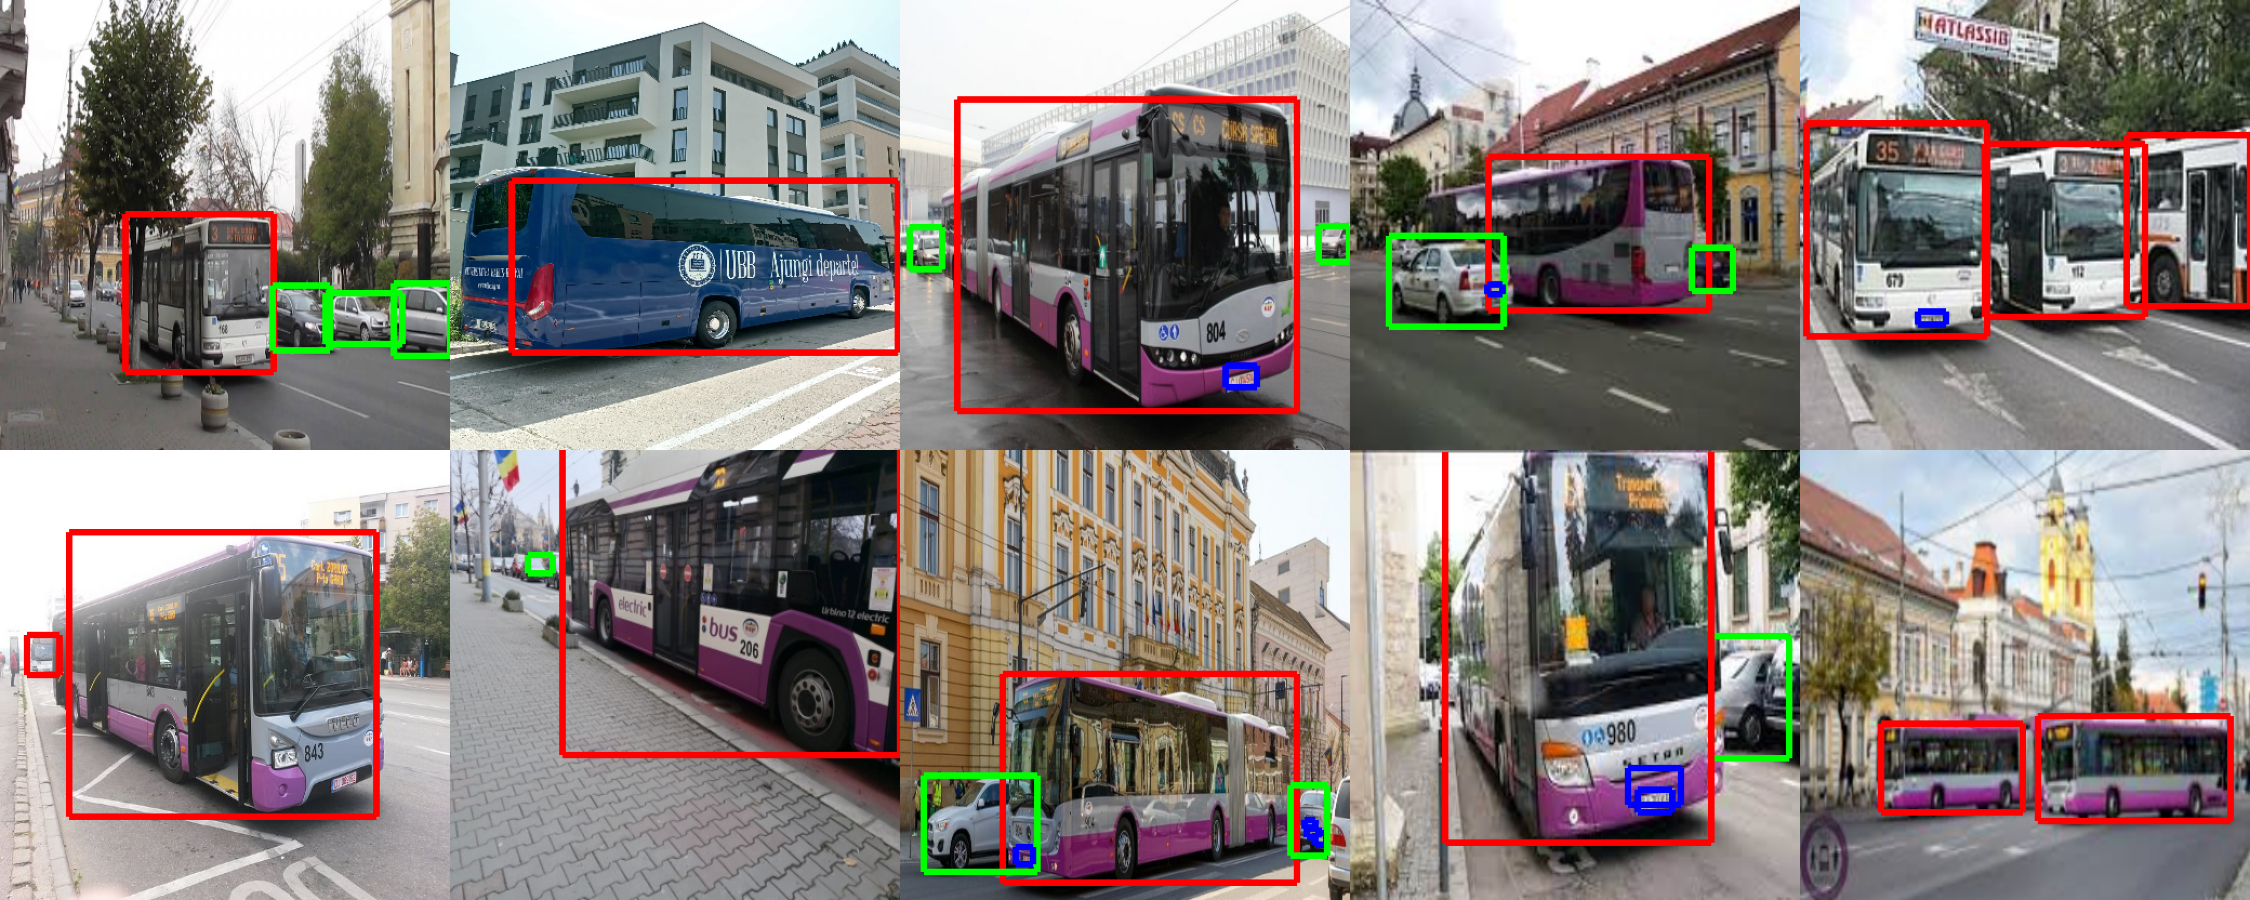
\includegraphics[scale=0.1]{images/cover.png}
        \caption{Images from Cluj-Napoca}
        \label{cluj}
    \end{figure}
    

    \def \scalevartuning {0.3}
    
    \begin{figure*}[htp] 
    %\centering
    \subfloat[mAP]{%
        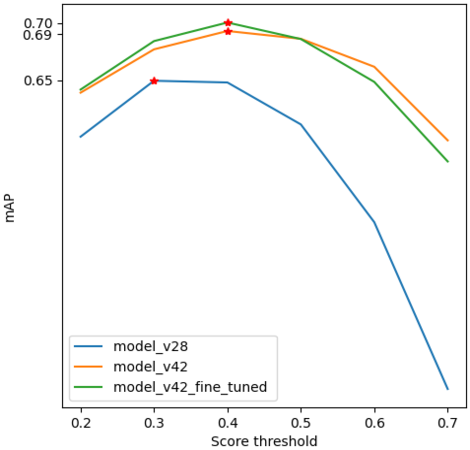
\includegraphics[scale=\scalevartuning]{images/final_mAP.png}%
        \label{mAP_final}%
        }%
    \hfill%
    \subfloat[Bus]{%
        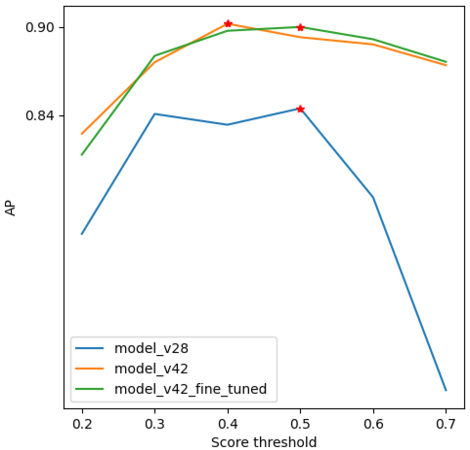
\includegraphics[scale=\scalevartuning]{images/final_bus.png}%
        \label{bus_final}%
        }%
    \hfill%
    \subfloat[Car]{%
        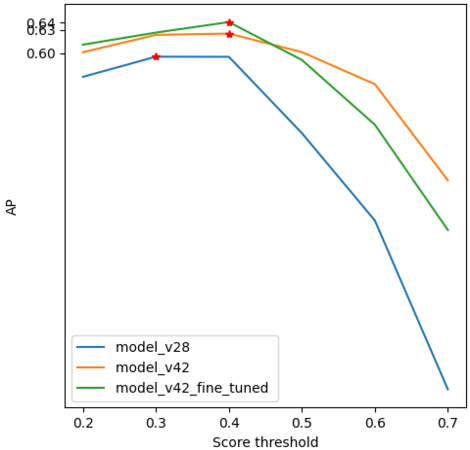
\includegraphics[scale=\scalevartuning]{images/final_car.png}%
        \label{car_final}%
        }%
     \hfill%
    \subfloat[License plate]{%
        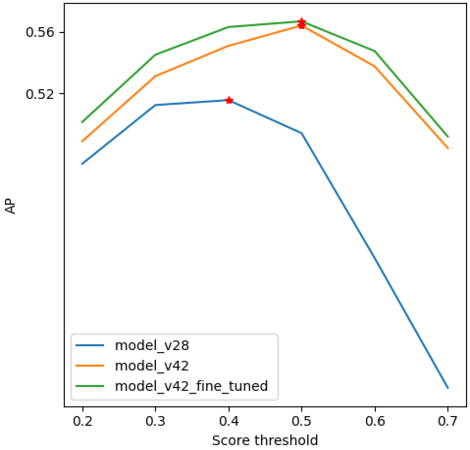
\includegraphics[scale=\scalevartuning]{images/final_license.png}%
        \label{license_final}%
        }%
    \caption{AP and mAP for the final model (orange), the model before hyperparameter tuning (blue), and the model after fine-tuning (green)}
    \label{curve_final}
    \end{figure*}



    To compute the exact improvements, we consider the maximum value from the mAP curve in Fig. \ref{curve_final}. We detail the exact improvements after hyperparameter tuning, in percents, in Table \ref{improvement_values}. 
    
    \begin{table}[H]
    \centering
    \caption{Improvement after hyperparameter tuning in percents for each class in AP and mAP for the average case}
    \begin{tabular}{c|c|c|c|c}
    Class         & Car     & Bus     & License plate & Average \\ \hline
    Before tuning & 59.52\% & 84.07\% & 51.25\%       & 64.95\% \\ \hline
    After tuning  & 62.54\% & 90.23\% & 55.09\%       & 69.29\% \\ \hline
    Improvement   & $3.02\% \uparrow$    & $6.16\% \uparrow$    & $3.84\% \uparrow$          & $4.34\% \uparrow$    
    \end{tabular}
    
    \label{improvement_values}
    \end{table}
    
    After tuning the hyperparameters, we perform fine tuning, meaning that we unfreeze the backbone of the model and further train with a very small learning rate. For fine tuning, we have used $\eta_{max}=10^{-5}$ and $\eta_{min}=10^{-8}$. 
    
    In Fig. \ref{curve_final} we can see that we achieved small improvements only by fine tuning and in Table \ref{improvement_values_finetuning} we detail the exact values obtained and the improvements. For the bus class there is a slight decrease, but in general the improvements are positive.

    \begin{table}[h]
    \centering
      \caption{Improvement after fine tuning in percents for each class in AP and mAP for the average case}
    \begin{tabular}{c|c|c|c|c}
    Class              & Car     & Bus     & License plate & Average \\ \hline
    Before fine tuning & 62.54\% & 90.23\% & 55.09\%       & 69.29\% \\ \hline
    After fine tuning  & 64.04\% & 90.01\% & 56.68\%       & 70.03\% \\ \hline
    Improvement        & $1.5\% \uparrow$   & $0.22\% \downarrow$ & $1.59\% \uparrow$        & $0.74\% \uparrow$ 
    \end{tabular}
  
    \label{improvement_values_finetuning}
    \end{table}
    
    
    
    In terms of speed, our solution achieves approximately 5 FPS on a Samsung A70 mobile phone.
    
    We present the result on some images from Cluj-Napoca in Fig. \ref{cluj}. Green bounding boxes represent cars, red bounding boxes represent buses, and blue bounding boxes represent registration plates.
    
